\documentclass[10pt,a4paper]{article}
\usepackage{amsmath,amssymb,amsthm,graphicx}
\usepackage{amsmath,amssymb,amsthm,graphicx}
\usepackage[no-math]{fontspec}
\newenvironment{authorclaim}[1]{\par\medskip\noindent\textbf{#1.}\ \ignorespaces}{\par\medskip}
\allowdisplaybreaks
\title{Hard k-CNF instances for PPSZ with small resolution width and near-2/k savings upper bound}
\author{Dominik Scheder, Navid Talebanfard}
\date{doi:10.4230/LIPIcs.CCC.2020.3; CC BY 3.0 Unported}
\begin{document}
\maketitle
\noindent\textit{Editorial scope.} Single main mechanism: hard instances and bounded-width PPSZ success upper bound. Supporting graph/width/game lemmas, parameter consequences and common-lift proof grouped once. Source's own final density/padding detail omission preserved; no author proof repair, extra assumptions, unconditional ETH/SETH claim or new conjecture.\par\medskip
\noindent\textit{Allowed standard prerequisites (editorial).}\begin{itemize}
\item Large-girth regular graphs, Hall's theorem and the Atserias-Dalmau resolution-width game characterization. Formal Erdős–Sachs[4] regular-graph existence and Atserias–Dalmau Theorem9[2] remain cited standard prerequisites. The paper's common-lift proof is completely retained in AppendixA rather than merely cited. All12 original bibliography entries retained.
\end{itemize}\medskip
\section*{PPSZ and width-bounded proof heuristics (Introduction)}
The PPSZ algorithm for $k$-SAT by Paturi, Pudl\'ak, Saks, and Zane [7] is simple to state but famously difficult to analyze. Given a $k$-CNF formula $\Phi$ as input, it first chooses a random ordering $\pi$ of its variables $x_1,\ldots,x_m$. It goes through them one by one, in the order given by $\pi$. For each variable $x$, it tries to derive the correct value using a certain proof heuristic $P$. $P$ takes as input a $k$-CNF formula $\Phi$ and a variable $x$ and returns a value in $\{0,1,?\}$. $P$ must be sound, meaning if $P(\Phi,x)=b\in\{0,1\}$ then $\Phi\models(x=b)$, i.e., every satisfying assignment of $\Phi$ sets $x$ to $b$; however, we allow $P$ to be incomplete, i.e., it may answer "?", meaning "I don't know". If $P(\Phi,x)=b\in\{0,1\}$, then PPSZ sets $x$ to $b$; otherwise it sets $x$ to some $b\in\{0,1\}$ chosen uniformly at random. In either case, it simplifies $\Phi$ to $\Phi|_{x\mapsto b}$. Once all variables have been processed, the resulting formula either contains the empty clause $\square$, and we declare this run of PPSZ a failure; or it does not, in which case PPSZ has found a satisfying assignment.
If PPSZ has success probability $p$ then we can repeat it $1/p$ times, obtaining a constant success probability. As long as $P$ runs in subexponential time, the overall running time of this Monte Carlo algorithm is dominated by $1/p$ (which will, most likely, be exponential in $n$). Which proof heuristics $P$ should one consider? There are currently just two on the market. The first one is $P_w$, which checks whether $(x=b)$ is implied by a set of up to $w$ clauses of $\Phi$. The second one is $R_w$, which tries to derive the clause $(x=b)$ by resolution, bounded by width $w$. Obviously they both can be implemented in time $O^*(\binom{|\Phi|}{w})\le O^*(\binom{m^k}{w})$, which is subexponential as long as $w\in o(m/\log m)$. It is easy to see that $R_{w\cdot k}$ is at least as strong as $P_w$. We also speak of weak PPSZ when it uses $P_w$ and strong PPSZ when it uses $R_w$ (ignoring the concrete values of $w$).
\section*{2.1 Notation}
Given a set of variables $X$, a partial assignment is a function $\alpha:X\to\{0,1,*\}$, that is an assignment of 0-1 values to some of the variables with $*$ intended to mean unset by $\alpha$. We denote the set of variables to which $\alpha$ gives a value by $\operatorname{var}(\alpha):=\{x\in X:\alpha(x)\in\{0,1\}\}$. For two partial assignments $\alpha$ and $\beta$ we write $\alpha\subseteq\beta$ to mean that for every $x\in\operatorname{var}(\alpha)$, it holds that $\beta(x)=\alpha(x)$. Naturally, $\alpha\subset\beta$ means that $\alpha\subseteq\beta$ and $|\operatorname{var}(\alpha)|<|\operatorname{var}(\beta)|$. Given a variable $x$ and $b\in\{0,1\}$, $x\mapsto b$ is the partial assignment which sets $x$ to $b$. The assignment which sets every variable to0 is denoted by $\mathbf0$. For $Y\subseteq X$, we write $Y\mapsto0$ to denote the partial assignment which sets all variables in $Y$ to0. If $\operatorname{var}(\alpha)\cap\operatorname{var}(\beta)=\varnothing$, we define $\alpha\cup\beta$ to be the partial assignment which sets all $x\in\operatorname{var}(\alpha)$ to $\alpha(x)$, all $x\in\operatorname{var}(\beta)$ to $\beta(x)$, and all other variables to $*$. Finally the restriction of a formula $\Phi$ by $\alpha$ is denoted by $\Phi|_\alpha$.

\section*{2 Our Results}
\begin{authorclaim}{Theorem 2 (SSETH Holds for PPSZ)}
For every $k\in\mathbb N$, there is a polynomial $p$ and a sequence $(F_m)_{m\in\mathbb N}$ of satisfiable $k$-CNF formulas $F_m$ on $m$ variables, such that for every $\epsilon>0$ and
\[
w\le\sqrt{\epsilon\cdot\frac{\log\log m}{2\log k}}-3,
\]
it holds that
\[
\Pr[\operatorname{ppsz}(F_m,R_w)\text{ succeeds}]
\le p(m)2^{-m(1-2(1+\epsilon)/k)}.
\]
\end{authorclaim}
Thus, the super strong exponential time hypothesis is true for Strong PPSZ, provided that we do not make it too strong, i.e., keep $w$ fairly small. Note that this gives an upper bound on the savings of PPSZ by $2/k$, which is quite close to the currently best lower bound of $(\pi^2/6+o(1))/k$ [7].

\section*{2.2 The Formula}
Let $G=(V,E)$ be a graph. For every $e\in E(G)$ we introduce a variable $x_e$. Given a charge $c:V\to\{0,1\}$, the Tseitin formula on $G$ with charge $c$ is the Boolean formula
\begin{equation}
\operatorname{Tseitin}(G,c):=\bigwedge_{u\in V(G)}
\left(\sum_{e\in E(G):u\in e}x_e\equiv c(u)\pmod2\right).\tag{1}
\end{equation}
If $G$ has maximum degree $k$ then this can be expressed as a $k$-CNF formula on $m=|E(G)|$ variables and $|V(G)|2^{k-1}$ clauses. Usually in proof complexity, the charge $c$ is chosen so that $\operatorname{Tseitin}(G,c)$ is unsatisfiable. In this paper, all charges will be0, and $\operatorname{Tseitin}(G,0)$ is obviously satisfiable: set all variables to0. We will hence drop $c$ from the notation and simply write $\operatorname{Tseitin}(G)$ to denote this formula. The constraint $\sum_{e\in E(G):u\in e}x_e\equiv0\pmod2$ is called the Tseitin constraint of vertex $u$. Given a set $B$ of pairs of edges in $G$ consider the following formula
\[
\operatorname{Tseitin}(G)\wedge\bigwedge_{\{e,f\}\in B}(\bar x_e\vee\bar x_f).
\]
The constraint $(\bar x_e\vee\bar x_f)$ is called a bridge constraint. It is easy to see that $\mathbf0$ is the unique satisfying assignment of this formula if and only if every cycle in $G$ contains a bridge in $B$. We will consider a particular instantiation of bridges given by graph homomorphisms. A graph homomorphism from a graph $G$ to a graph $H$ is a function $\phi:V(G)\to V(H)$ such that $\{\phi(u),\phi(v)\}\in E(H)$ whenever $\{u,v\}\in E(G)$. Thus, $\phi$ also induces a function from $E(G)$ to $E(H)$; $\phi(\{u,v\}):=\{\phi(u),\phi(v)\}$. Given $G,H$, and a homomorphism $\phi$ from $G$ to $H$, we define a Tseitin formula with bridges on the variable set $\{x_e\mid e\in E(G)\}$:
\begin{equation}
\operatorname{TseitinBridge}(G,H,\phi):=
\operatorname{Tseitin}(G)\wedge
\bigwedge_{\substack{e,f\in E(G)\\e\ne f,\phi(e)=\phi(f)}}(\bar x_e\vee\bar x_f).\tag{2}
\end{equation}
For brevity, we write $V=V(G)$ and $E=E(G)$.
\begin{authorclaim}{Observation 5}
If $\operatorname{girth}(G)>|E(H)|$ then $\operatorname{TseitinBridge}(G,H,\phi)$ is uniquely satisfiable by $\mathbf0$.
\end{authorclaim}
\begin{proof}
Let $\alpha\ne\mathbf0$ be a total assignment. Let $F:=\{e\in E(G)\mid\alpha(x_e)=1\}$. If some vertex $u$ has degree1 in $(V,F)$, then $\alpha$ violates its Tseitin constraint. Otherwise, $(V,F)$ has a cycle, which has length at least $\operatorname{girth}(G)$. By the pigeonhole principle, this cycle contains two edges $e,f$ such that $\phi(e)=\phi(f)$, and thus $\alpha$ violates their bridge constraint.
\end{proof}
\paragraph{Locally Injective Homomorphisms}
A homomorphism $\phi$ is called locally injective if for every $u\in V(G)$ and any two of its neighbors $v_1$ and $v_2$, it holds that $\phi(v_1)\ne\phi(v_2)$. Note that $\phi:G\to H$ being locally injective immediately implies that $\deg_G(u)\le\deg_H(\phi(u))$. We call $\phi$ locally bijective if, additionally, $\deg_G(u)=\deg_H(\phi(u))$ for all vertices $u$ of $G$. Note that a locally bijective homomorphism bijectively maps the neighborhood of $u$ to the neighborhood of $\phi(u)$. The graph $G$ is called a covering graph of $H$ or a lift of $H$.
\begin{center}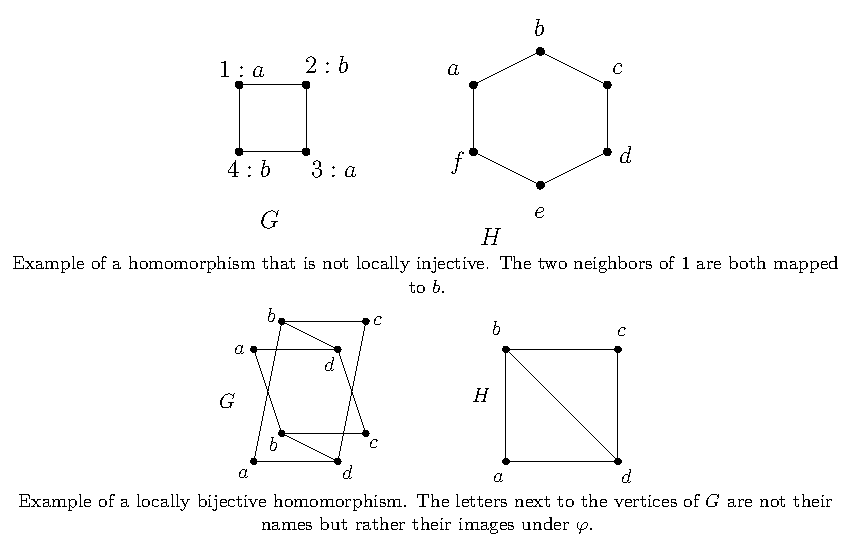
\includegraphics[width=.95\linewidth]{homomorphism-examples.pdf}\end{center}
\begin{authorclaim}{Theorem 6}
Let $G$ be a graph on $n$ vertices and $m$ edges. Suppose there is a locally injective graph homomorphism $\phi:G\to H$ for some graph $H$ with $|E(H)|<\operatorname{girth}(G)$. Then for all $\epsilon>0$ and $w:=\sqrt{\epsilon\cdot\operatorname{girth}(H)/2}-3$, the success probability of PPSZ with heuristic $R_w$ on $\Phi:=\operatorname{TseitinBridge}(G,H,\phi)$ is at most
\[
\Pr[\operatorname{ppsz}(\Phi,R_w)]\le2^{-m+(1+\epsilon)n}.
\]
\end{authorclaim}
\begin{proof}[Proof of Theorem2 using Theorem6]
We first show how to construct $F_m$ for infinitely many $m$. Let $n_0$ be some given, sufficiently large even integer. A well-known fact, first proven by Erd\H{o}s and Sachs [4], is that there is a $k$-regular graph $G_0$ on $n_0$ vertices having girth at least $g_0:=\log n_0/\log(k-1)$. Set $n_1:=\lfloor2(g_0-1)/k\rfloor$ or $n_1:=\lfloor2(g_0-1)/k\rfloor-1$, whichever is even, and let $G_1$ be a $k$-regular graph on $n_1$ vertices, such that $\operatorname{girth}(G_1)\ge g_1:=\log n_1/\log(k-1)$. This exists, provided that $n_0$ is sufficiently large. Note that $G_1$ has at most $g_0-1<\operatorname{girth}(G_0)$ edges.
A result by Angluin and Gardiner [1] states that there is a common lift $G$ of $G_0$ and $G_1$. That is, $G$ is a covering graph of $G_0$ and of $G_1$. Being a lift of a $k$-regular graph, $G$ is $k$-regular as well. A closer inspection of their proof reveals that $n:=|V(G)|\le4n_0n_1$.
Let $m:=kn/2$ be the number of edges in $G$. We set $\Phi_m:=\operatorname{TseitinBridge}(G,G_1,\phi_1)$, where $\phi_1$ is the locally bijective homomorphism from $G$ to $G_1$.
It is not difficult to see that lifting cannot decrease the girth, and thus $\operatorname{girth}(G)\ge\operatorname{girth}(G_0)>|E(G_1)|$. Thus, we can apply Theorem6 to $G,G_1$, and $\phi_1$, and conclude that the success probability of PPSZ on $\Phi_m$ is at most $2^{-m+(1+\epsilon)n}$ when using heuristic $R_w$. A quick calculation shows that $g_1\ge\log\log m/\log k$ if $n_0$ is sufficiently large, and thus
\[
w\ge\sqrt{\epsilon\cdot\frac{\log\log m}{2\log k}}-3.
\]
This construction gives us an infinite set $M\subseteq\mathbb N$ and, for each $m\in M$, a satisfiable $k$-CNF formula $F_m$ on $m$ variables for which the claimed hardness result holds. By a simple tweaking of the construction, we can ensure that $M$ is "reasonably dense", meaning that there is some $m^*\in M\cap[m-\log m,m]$ for all sufficiently large $m$. We then let $F_{m^*}$ be $F_m$, plus $m-m^*$ dummy variables. The success probability is then at most $2^{-m^*(1-2(1+\epsilon)/k)}\le\operatorname{poly}(m)2^{-m(1-2(1+\epsilon)/k)}$. We leave the details to the reader.
\end{proof}

\section*{3 All You Need to Know About PPSZ: Proof of Theorem6}
We will explain the connection between PPSZ and width-bounded resolution lower bounds. After this section, the reader can forget everything about PPSZ and think of this paper as proving a certain resolution width lower bound. If $C=(C'\vee x)$ and $D=(D'\vee\bar x)$ are clauses, then $(C'\vee D')$ is called the resolvent of $C$ and $D$. It is clear that $C\wedge D$ logically implies $C'\vee D'$. Let $\Phi$ be a CNF formula. A resolution derivation from $\Phi$ is a sequence of clauses $C_1,\ldots,C_t$ such that every $C_i$ is (1) a clause of $\Phi$ or (2) the resolvent of two earlier clauses. The width of the derivation is $\max_{1\le i\le t}|C_i|$. For a clause $C$, we denote by $\operatorname{width}(\Phi\vdash C)$ the minimum width of a resolution derivation from $\Phi$ that contains $C$. Resolution is complete for refutations, that is, $\Phi$ is unsatisfiable if and only if there is a derivation of the empty clause, denoted by $\square$, from $\Phi$.
\begin{proof}[Proof of Theorem6]
Let $G,H,\phi$ be as in Theorem6, and let $\Phi:=\operatorname{TseitinBridge}(G,H,\phi)$. The only satisfying assignment of $\Phi$ is $\mathbf0$. Consider a variant of PPSZ run on $\Phi$ such that whenever it has to pick a random value for a variable, it correctly sets it to0. Fix a permutation $\pi$. Let $Y(\pi)$ be the set of variables for which this variant of PPSZ under $\pi$ could not derive the value using $R_w$, and let $Z(\pi):=\operatorname{var}(\Phi)\setminus Y(\pi)$ be the rest, i.e., all variables whose value can be derived using $R_w$ once all variables before them in $\pi$ are set to0. It is not difficult to see that the success probability of the actual PPSZ on $\Phi$ is exactly $\mathbb E_\pi[2^{-|Y(\pi)|}]$.
Suppose, for the sake of contradiction, that PPSZ using heuristic $R_w$ has success probability greater than $2^{-m+(1+\epsilon)n}$. Then there is some $\pi$ for which $Z(\pi)\ge(1+\epsilon)n$. Fix this $\pi$ and set $Z:=Z(\pi)$ and $Y:=Y(\pi)$. The set of variables $Z$ corresponds to a set $F$ of edges, $F=\{e\in E(G):x_e\in Z\}$. Set $G'=(V,F)$. Note that $G'$ has $n$ vertices and at least $(1+\epsilon)n$ edges. Setting a variable in $\Phi$ to0 corresponds to simply deleting the corresponding edge in $G$, and therefore
\[
\Phi|_{Y\mapsto0}=\operatorname{TseitinBridge}(G',H,\phi).
\]
For a graph $G=(V,E)$ and a set $X\subseteq V$, define the edge boundary $\partial(X):=\{e\in E:|e\cap X|=1\}$. Call $G$ an $(a,b)$-expander if $|\partial(X)|\ge b$ for all sets $X$ of exactly $a$ vertices. The next lemma is basically Lemma17 from [9], adapted for our purposes. We give a proof for completeness.
\begin{authorclaim}{Lemma7}
Let $\epsilon>0$ and let $G'$ be a graph on $n$ vertices with at least $(1+\epsilon)n$ edges. Let $\ell\in\mathbb N$ and $h=\ell/\epsilon$. If $h<\operatorname{girth}(G')$ then $G'$ contains a non-empty subgraph $G''$ that has minimum degree at least2 and is an $(h,\ell+1)$-expander.
\end{authorclaim}
\begin{proof}
Start with $G''=G'$. If $G''$ has a vertex of degree0 or1, delete it. If $G''$ contains a set $X$ of $h$ vertices with $|\partial(X)|\le\ell$, delete $X$ from $G''$, along with all incident edges.
The first type of deletion removes one vertex and at most one edge. The second type removes exactly $h$ vertices. There are at most $\ell$ edges in the boundary of $X$; since $|X|<\operatorname{girth}(G')$, the graph $G''[X]$ is a forest, and thus there are at most $h-1$ edges within $X$. Thus, removing $X$ removes at most $\ell+h-1<(1+\epsilon)h$ edges.
We see that a step that removes $a$ vertices removes fewer than $(1+\epsilon)a$ edges. Suppose the process terminates with $t$ vertices deleted. Trivially $t\le n$. Fewer than $(1+\epsilon)n$ edges have been deleted, so $G''$ is non-empty.
\end{proof}
Let $G''$ be given by Lemma7 with $\ell:=w+1$. We will further restrict $\Phi$ so that only edges of $G''$ remain unset. Let $F'':=E(G)\setminus E(G'')$, $Y'':=\{x_e:e\in F''\}$, and $\Phi'':=\Phi|_{Y''\mapsto0}$. Note that $\Phi''=\operatorname{TseitinBridge}(G'',H,\phi)$. Recall that all edges of $G''$ are mentioned in $Z$ and since $Y''\supseteq Y$ and restricting additional variables cannot increase the resolution width, we conclude that there exists $e\in E(G'')$ such that
\begin{equation}
\operatorname{width}(\Phi''\vdash\bar x_e)\le w.\tag{3}
\end{equation}
Towards a contradiction, we claim that in fact this resolution width is large for all variables $x_e$ where $e\in E(G'')$. Indeed, we have the following theorem:
\begin{authorclaim}{Theorem8 (Resolution Lower Bound)}
Let $G$ be a graph of minimum degree2 that is an $(h,\ell+1)$-expander. Suppose there is a locally injective homomorphism $\phi:G\to H$ into some graph $H$. Then
\begin{equation}
\operatorname{width}(\operatorname{TseitinBridge}(G,H,\phi)\vdash\bar x_e)>\ell-1,\tag{4}
\end{equation}
for all edges $e$ of $G$, provided that $2h\ell+5h+\ell<\operatorname{girth}(H)$.
\end{authorclaim}
Note that $G''$ has minimum degree2 and is a $(h,\ell+1)$-expander for $\ell=w+1$ and $h=(w+1)/\epsilon$. Also note that $\phi:V(G'')\to V(H)$ (or rather, the restriction of $\phi$ to $V(G'')$) is still a locally injective homomorphism. Recall that $w=\sqrt{\epsilon\cdot\operatorname{girth}(H)/2}-3$ and hence $2h\ell+5h+\ell=2(w+1)^2/\epsilon+5(w+1)/\epsilon+w+1<\operatorname{girth}(H)$, and thus Theorem8 applies to $G''$. This contradicts(3) and finishes the proof of Theorem6.
\end{proof}

\section*{4 Proof of Theorem8}
Let $\Phi=\operatorname{TseitinBridge}(G,H,\phi)$ and let $e^*$ be an edge of $G$. We will show that $\operatorname{width}(\Phi\vdash\bar x_{e^*})>\ell-1$ for all such edges $e^*$. In fact, we will prove $\operatorname{width}(\Phi|_{x_{e^*}\mapsto1}\vdash\square)>\ell-1$, which is a slightly stronger statement.
We will use the game characterization of resolution width due to Atserias and Dalmau [2]. Given a CNF formula $F$, the $\ell$-bounded Atserias-Dalmau game played by two players, Prover and Delayer is defined as follows. A position in this game is a partial assignment $\alpha$ setting up to $\ell$ variables. The start position is the empty assignment. At position $\alpha$, Prover can either (1) forget some variables, i.e., replace $\alpha$ by some $\beta\subset\alpha$. Or, (2), if $|\operatorname{var}(\alpha)|\le\ell-1$, pick a variable $x\notin\operatorname{var}(\alpha)$ and query it; Delayer has to respond with a truth value $b\in\{0,1\}$, and $\alpha$ is updated to $\alpha\cup(x\mapsto b)$. The game ends if $\alpha$ violates a clause of $F$, in which case Prover wins. Delayer wins if she has a strategy to play indefinitely.
\begin{authorclaim}{Theorem9 (Atserias and Dalmau [2])}
Let $F$ be an unsatisfiable CNF formula. If Delayer has a winning strategy for the $\ell+1$-bounded game then there is no width-$\ell$ resolution refutation of $F$.
\end{authorclaim}
To show that $\operatorname{width}(\Phi|_{x_{e^*}\mapsto1}\vdash\square)>\ell-1$ we define a winning strategy for Delayer for the $\ell$-bounded game that ensures she never loses. Indeed, we will modify the game a bit: it is now played on $\Phi$ instead of $\Phi|_{x_{e^*}\mapsto1}$; the starting position is the partial assignment $x_{e^*}\mapsto1$; Prover can never forget $x_{e^*}$ but is now allowed partial assignments up to size $\ell+1$. That is, he can query a new variable provided $|\operatorname{var}(\alpha)|\le\ell$. It is easy to see that if Delayer wins this modified game, she wins the original one, too. Since $\Phi=\operatorname{TseitinBridge}(G,H,\phi)$, we can easily rephrase the rules of the game in terms of sets of edges instead of partial assignments:
\begin{quote}
\textbf{The Atserias-Dalmau, Graph View.} A position of the game is described by two disjoint set $F_0,F_1\subseteq E(G)$. $F_0$ and $F_1$ correspond to the variables of $\Phi$ that the current partial assignment sets to0 and1, respectively. The start position is $F_0=\varnothing$ and $F_1=\{e^*\}$.
In every step, Prover either (1) removes one edge $e$ from $F_0$ or $F_1$ (but never removes $e^*$). Or (2) he queries an edge $e\in E(G)\setminus(F_0\cup F_1)$, provided $|F_0|+|F_1|\le\ell$. Delayer can then decide whether to add $e$ to $F_0$ or $F_1$.
Prover wins if there is a vertex $u$ in $G$ such that all edges incident to $u$ are in $F_0\cup F_1$ but $\deg_{F_1}(u)$ is odd (then the partial assignment $\alpha$ violates the Tseitin constraint of $u$); or if there are two edges $e,f\in F_1$ with $\phi(e)=\phi(f)$ (then $\alpha$ violates a bridge constraint).
\end{quote}
We will now describe a winning strategy for Delayer. Throughout the game, she maintains a set $\widetilde F_1$ such that $F_1\subseteq\widetilde F_1\subseteq E\setminus F_0$. Let $V(\widetilde F_1)$ denote the set of vertices incident to at least one edge of $\widetilde F_1$. She makes sure $\widetilde F_1$ satisfies certain invariants:
\begin{enumerate}
\item Every connected component of $(V,\widetilde F_1)$ is a path; a path of positive length (i.e., a path that is not an isolated vertex) is called an $\widetilde F_1$-path.
\item Every $\widetilde F_1$-path contains at least one edge of $F_1$.
\item $\phi$ is injective on $V(\widetilde F_1)$.
\item Each $\widetilde F_1$-path has length at least $2h+1$, and the first and last $h$ edges of every $\widetilde F_1$-path are not in $F_1$.
\item Each $\widetilde F_1$-path has length at most $2h\ell+2h+\ell$.
\end{enumerate}
\begin{authorclaim}{Observation10}
If $\widetilde F_1$ satisfies the invariants, then no constraint is violated.
\end{authorclaim}
\begin{proof}
In fact we show that invariants1–4 already give the result. First, consider a Tseitin constraint of a vertex $u$. Since $\widetilde F_1$ consists of disjoint paths, so does $F_1$. Thus, $u$ is incident to0,1, or2 edges of $F_1$. If it is incident to0 or2 edges of $F_1$, the Tseitin constraint of $u$ is clearly not falsified. If it is incident to exactly one edge of $F_1$, then it is the endpoint of some path of $F_1$-edges. By Invariant4, $u$ is incident to some other edge $f\in\widetilde F_1\setminus F_1$. Thus, $f$ is neither in $F_0$ nor in $F_1$, and the Tseitin constraint of $u$ is not violated.
Next, consider a bridge constraint $(\bar x_e\vee\bar x_f)$. By construction we have $\phi(e)=\phi(f)$. By Invariant3, $\phi$ is injective on $\widetilde F_1$, and thus $e,f$ cannot both be in $F_1$, and the bridge constraint is not violated.
\end{proof}
We will use the following property of $\phi$.
\begin{authorclaim}{Proposition11}
Let $G'$ be a connected subgraph of $G$ of diameter less than $\operatorname{girth}(H)$. Then $\phi$ is injective on $V(G')$, and thus $\phi(G')$ is isomorphic to $G'$.
\end{authorclaim}
\begin{proof}
For the sake of contradiction, suppose $u,v\in V(G')$ are two vertices with $\phi(u)=\phi(v)$. Let $p$ be a shortest path from $u$ to $v$ in $G'$. Write $p$ as $u=u_0,u_1,\ldots,u_t=v$. By assumption, $t<\operatorname{girth}(H)$. Under $\phi$, the path $p$ is mapped to a reduced walk in $H$, reduced meaning that $\phi(u_{i-1})\ne\phi(u_{i+1})$ for all $1\le i\le t-1$. Since $\phi(u)=\phi(v)$, this is a closed walk and thus contains a cycle. The cycle has length at most $t<\operatorname{girth}(H)$, a contradiction.
\end{proof}
\paragraph{How to initialize $\widetilde F_1$}
Delayer can easily initialize $\widetilde F_1$. Write $e^*=\{u^*,v^*\}$. Since $G$ has minimum degree2, Delayer can start a reduced walk from $u^*$ of length $h$, and also from $v^*$ and add this to $\widetilde F_1$. Since $2h+1<\operatorname{girth}(H)$, this is a path; by Proposition11, $\phi$ is injective on its vertices.
\paragraph{How to handle a Forget Step}
Suppose Prover forgets some edge $e\in F_0\cup F_1$. If $e\in F_0$, Delayer leaves $\widetilde F_1$ unchanged. If $e\in F_1$, let $p$ be the $\widetilde F_1$-path containing $e$. If $p$ contains some other $F_1$-edge besides $e$, Delayer does not change $\widetilde F_1$; otherwise it simply removes all of $p$ from $\widetilde F_1$. All invariants stay satisfied.
\paragraph{How to handle a Query from Prover}
Suppose Prover queries an edge $e$. Delayer has now to choose whether to include $e$ into $F_0$ or $F_1$, and potentially update $\widetilde F_1$.
\paragraph{Case1: $e$ is not in $\widetilde F_1$}
Then Delayer adds $e$ to $F_0$ and leaves $\widetilde F_1$ unchanged. All invariants still hold. This includes the case that $e$ is incident to some vertex on a $\widetilde F_1$-path, but is not itself inside this path.
\paragraph{Case2: $e$ is in some $\widetilde F_1$-path $p$ but not among its first or last $h$ edges}
Delayer adds $e$ to $F_1$ and leaves $\widetilde F_1$ unchanged. All invariants still hold.
\paragraph{Case3: $e$ is among the first or last $h$ edges of some $\widetilde F_1$-path $p$}
Let $v_1,\ldots,v_{h+1}$ be the first $h+1$ vertices of $p$, and let $q$ denote the length-$h$-path $v_1,\ldots,v_{h+1}$. By assumption, $e$ lies on the path $q$. Since $G$ is an $(h,\ell+1)$-expander, there are edges $f_1,\ldots,f_{\ell+1}$, each incident to exactly one vertex in $\{v_1,\ldots,v_h\}$. One of those edges could be $\{v_h,v_{h+1}\}$, but without loss of generality, for $1\le i\le\ell$, edge $f_i$ connects some $a_i\in\{v_1,\ldots,v_h\}$ to some $b_i$ outside $\{v_1,\ldots,v_{h+1}\}$. Since $G$ has minimum degree2 and girth larger than $h$, we can find paths $p_1,\ldots,p_\ell$ such that each $p_i$ has length $h$ and starts with $a_i$ as its first and $b_i$ as its second vertex. Since $3h<\operatorname{girth}(H)\le\operatorname{girth}(G)$, the $p_i$ are vertex-disjoint. Since $h+|p|\le h+2h\ell+2h+\ell<\operatorname{girth}(H)\le\operatorname{girth}(G)$, the path $p_i$ intersects $p$ only in vertex $a_i$. Thus, $C:=p\cup p_1\cup\cdots\cup p_\ell$ is a tree, and its diameter is at most $h+2h\ell+2h+\ell$. This figure shows how $C$ could look like:
\begin{center}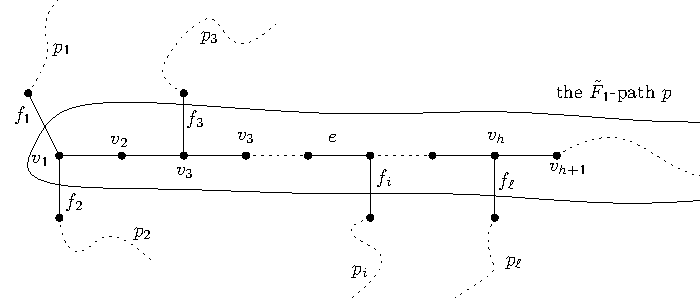
\includegraphics[width=.92\linewidth]{delayer-branches.pdf}\end{center}
Call $p_i$ blocked by $F_0$ if it contains some edge from $F_0$; at most $|F_0|$ of the $\ell$ paths are blocked by $F_0$. Let $p'$ be an $\widetilde F_1$-path different from $p$. We say $p'$ blocks $p_i$ if the vertex sets of $\phi(p')$ and $\phi(p_i)$ intersect.
\begin{authorclaim}{Proposition12}
Let path $p'$ in $\widetilde F_1$ be different from $p$. Then $p'$ blocks at most one of the paths $p_1,\ldots,p_\ell$.
\end{authorclaim}
\begin{proof}
Let $C=p\cup p_1\cup\cdots\cup p_\ell$. As argued above, this is a tree in $G$ and its diameter is less than $\operatorname{girth}(H)$. By Proposition11, its image $\phi(C)$ is a tree in $H$, isomorphic to $C$. Suppose, for the sake of contradiction, that $\phi(p')$ intersects $\phi(p_i)$ and $\phi(p_j)$. This scenario would look like this:
\begin{center}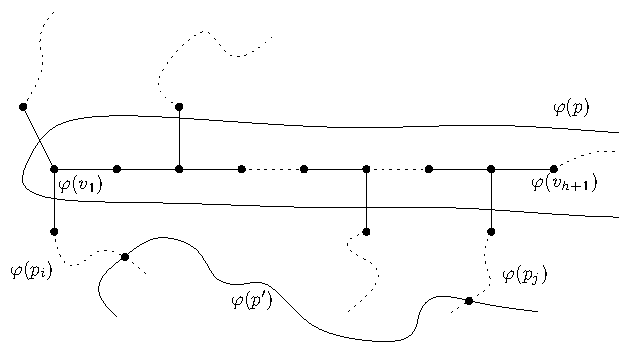
\includegraphics[width=.85\linewidth]{blocking-cycle.pdf}\end{center}
Since $\phi(p')$ and $\phi(p)$ do not share any vertex (by Invariant3), the subgraph $\phi(p')\cup\phi(p_i)\cup\phi(p_j)\cup\phi(p)$ contains a cycle. This cycle has size at most $|p'|+|p_i|+|p_j|+|q|\le2h\ell+2h+\ell+3h$, a contradiction.
\end{proof}
Call $p_i$ blocked by $\widetilde F_1$ if there is some $\widetilde F_1$-path different from $p$ that blocks $p_i$. By Proposition12, at most $|F_1|-1$ paths $p_i$ are blocked by $\widetilde F_1$. Thus, a total of at most $|F_0|+|F_1|-1\le\ell-1$ of the paths $p_i$ are blocked by $F_0$ or $\widetilde F_1$. Thus, there exists some path $p_i$, $1\le i\le\ell$, that is not blocked. We now modify $p$ by removing the edges on the path $v_1,v_2,\ldots,a_i$ and adding $p_i$. Let $\hat p$ denote the new version of $p$ and $\hat F_1$ the new version of $\widetilde F_1$. Note that $F_1\subseteq\hat F_1$ still holds, since we only modify the set $\widetilde F_1\setminus F_1$. Obviously, $\hat F$ satisfies Invariants1,2, and4. Since $p_i$ is not blocked by $F_0$, $\hat F$ is disjoint from $F_0$; because $p_i$ is not blocked by $\widetilde F_1$, Invariant3 still holds. Invariant5 might be violated: $\hat p$ might be too long. We will deal with this in a minute.
Note that $e$ is now either outside $\hat F_1$, and Delayer can include it into $F_0$; or it is inside $\hat p$, but then it is not among the first or last $h$ edges of $\hat p$, and Delayer can include it into $F_1$.
It remains to address the possibility that $\hat p$ is too long, violating Invariant5. If indeed $\hat p$ has more than $2h\ell+2h+\ell$ edges, then it must somewhere contain $2h+1$ consecutive edges that are not in $F_1$ (note that $|F_1|\le\ell$). Let $e_0,\ldots,e_{2h}$ be these edges. Define $\hat F_1:=\widetilde F_1\setminus\{e_h\}$. That is, we split $\hat p$ into two parts, the first ending in $e_0,\ldots,e_{h-1}$, the second starting with $e_{h+1},\ldots,e_{2h}$. Note that this satisfies Invariant4. If one of these paths contains no edge from $F_1$ at all, we delete it from $\hat F$. We continue this process until all paths in $\hat F$ have size at most $2h\ell+2h+\ell$. The final $\hat F$ satisfies all invariants.

\section*{A Existence of Common Lift}
\begin{authorclaim}{Theorem13 (Angluin and Gardiner [1])}
Let $G$ and $H$ be $k$-regular graphs. Then there exists a $k$-regular graph $L$ that is a common lift of both $G$ and $H$. Furthermore, $|V(L)|\le4|V(G)|\cdot|V(H)|$.
\end{authorclaim}
\begin{proof}
Suppose first that both $G=(U,E)$ and $H=(V,F)$ are bipartite. By Hall's Theorem, each has a perfect matching, and in fact, we can partition $E$ and $F$ into $k$ perfect matchings each: $E=E_1\uplus\cdots\uplus E_k$ and $F=F_1\uplus\cdots\uplus F_k$. The common lift $L$ has vertex set $U\times V$ and edge set
\[
\bigcup_{i=1}^k\left\{\{(u,v),(u',v')\}\in\binom{U\times V}{2}\mid\{u,u'\}\in E_i,\{v,v'\}\in F_i\right\}.
\]
It is not difficult to see that the projections $\phi_G:(u,v)\mapsto u$ and $\phi_H:(u,v)\mapsto v$ are locally bijective homomorphisms from $L$ into $G$ and $H$, respectively.
If $G$ (or $H$ or both) fails to be bipartite, we first replace it by its 2-lift $G_2$. The vertex set of $G_2$ is $U\times\{0,1\}$, and we form its edge set by creating, for each $\{u,v\}\in E$, two edges $\{(u,0),(v,1)\}$ and $\{(u,1),(v,0)\}$. The graph $G_2$ is bipartite, and projection to the first coordinate is a locally bijective homomorphism. Finally, observe that the composition of locally bijective homomorphisms is again a locally bijective homomorphism. Altogether, we can replace $G$ and $H$ by their respective 2-lifts $G_2$ and $H_2$; these are bipartite graphs, so we find a common lift $L$ on $4|U|\cdot|V|$ vertices.
\end{proof}

\begin{thebibliography}{12}
\bibitem{r1} Dana Angluin and A Gardiner. Finite common coverings of pairs of regular graphs. Journal of Combinatorial Theory, Series B, 30(2):184–187, 1981. doi:10.1016/0095-8956(81)90062-9.
\bibitem{r2} Albert Atserias and Víctor Dalmau. A combinatorial characterization of resolution width. J. Comput. Syst. Sci., 74(3):323–334, 2008. doi:10.1016/j.jcss.2007.06.025.
\bibitem{r3} Shiteng Chen, Dominik Scheder, Navid Talebanfard, and Bangsheng Tang. Exponential lower bounds for the PPSZ k-SAT algorithm. In Sanjeev Khanna, editor, Proceedings of the Twenty-Fourth Annual ACM-SIAM Symposium on Discrete Algorithms, SODA 2013, New Orleans, Louisiana, USA, January 6-8, 2013, pages 1253–1263. SIAM, 2013. doi: 10.1137/1.9781611973105.91.
\bibitem{r4} Paul Erdős and Horst Sachs. Reguläre graphen gegebener taillenweite mit minimaler knotenzahl. (regular graphs with given girth and minimal number of knots.). Wiss. Z. Martin-Luther-Univ. Halle-Wittenberg, Math.-Naturwiss., 12:251–258, 1963.
\bibitem{r5} Thomas Dueholm Hansen, Haim Kaplan, Or Zamir, and Uri Zwick. Faster k-sat algorithms using biased-ppsz. In Moses Charikar and Edith Cohen, editors, Proceedings of the 51st Annual ACM SIGACT Symposium on Theory of Computing, STOC 2019, Phoenix, AZ, USA, June 23-26, 2019, pages 578–589. ACM, 2019. doi:10.1145/3313276.3316359.
\bibitem{r6} Timon Hertli. 3-SAT faster and simpler - unique-SAT bounds for PPSZ hold in general. SIAM J. Comput., 43(2):718–729, 2014. doi:10.1137/120868177.
\bibitem{r7} Ramamohan Paturi, Pavel Pudlák, Michael E. Saks, and Francis Zane. An improved exponential-time algorithm for k-SAT. J. ACM, 52(3):337–364, 2005. doi:10.1145/1066100. 1066101.
\bibitem{r8} Ramamohan Paturi, Pavel Pudlák, and Francis Zane. Satisfiability coding lemma. Chicago J. Theor. Comput. Sci., 1999, 1999.
\bibitem{r9} Pavel Pudlák, Dominik Scheder, and Navid Talebanfard. Tighter hard instances for PPSZ. In 44th International Colloquium on Automata, Languages, and Programming, ICALP 2017, July 10-14, 2017, Warsaw, Poland, pages 85:1–85:13, 2017. doi:10.4230/LIPIcs.ICALP.2017.85.
\bibitem{r10} Dominik Scheder. PPSZ for $k\ge5$: More is better. TOCT, 11(4):25:1–25:22, 2019. doi: 10.1145/3349613.
\bibitem{r11} Uwe Schöning. A probabilistic algorithm for k-SAT and constraint satisfaction problems. In 40th Annual Symposium on Foundations of Computer Science, FOCS ’99, 17-18 October, 1999, New York, NY, USA, pages 410–414. IEEE Computer Society, 1999. doi:10.1109/ SFFCS.1999.814612.
\bibitem{r12} Nikhil Vyas and R. Ryan Williams. On super strong ETH. In Theory and Applications of Satisfiability Testing - SAT 2019 - 22nd International Conference, SAT 2019, Lisbon, Portugal, July 9-12, 2019, Proceedings, pages 406–423, 2019. doi:10.1007/978-3-030-24258-9\_28.
\end{thebibliography}
\end{document}
